%!TEX root = ../sample-acmlarge.tex
Although the IREOS index was the first, and so far the only, internal index devoted to bridging the gap related to the internal evaluation of outlier detection results \cite{zimek2013,marques2015}, it has the main limitation of restricting to directly evaluate only top-$n$ (binary) outlier detection results $\mathbf{S}$. Without previously know the number of outliers in the dataset $n$, it is not possible to evaluate a solution given as outlier scoring $\mathbf{y}$. In this section, we devise means to extend IREOS to evaluate a collection of candidate solutions $\mathbf{y}$ in the absence of labels and independent of a choice of $n$.

\subsection{Internal Evaluation of Top-n Outlier Detection Results}
Since the observations $\mathbf{x}_i$ are sorted and ranked according to their degree of outlierness $y_i$ and the threshold in the ranking is established, the top-$n$ observations can be labeled as outliers. Even though it is clear that the best solution must rank all outliers before all inliers and the worst solution must rank all inliers before all outliers, there are $n!$ different possible best top-$n$ solutions equally well rated. However, the truly best outlier solution should rank more obvious or clear outliers before less obvious outliers before those that could be outliers or inliers and so on. This issue was already discussed and addressed by \cite{schubert2012} in the context of the external evaluation of outlier detection, once that the main external measures (\textit{e.g.} ROC AUC and $prec@n$) cannot make such distinction. As well as these external measures, IREOS cannot differentiate the quality of these $n!$ different possible best solutions.

We start the IREOS extension addressing the problem discussed above, in order to make possible distinguish the quality of the ranks among the top-$n$ observations, we introduced weights in the Equation \ref{eq:ireos:avg_curve} where the average curve of separability is defined, so that the average curve of separability becomes a weighted average curve of separability,
\begin{equation}
\int_{\gamma = 0}^{\gamma_{max}} \bar{p}(\gamma) = \int_{\gamma = 0}^{\gamma_{max}} \frac{1}{\sum_{\mathbf{x}_i \in \mathbf{S}} w_i} \sum_{\mathbf{x}_i \in \mathbf{S}} p(\mathbf{x}_i, \gamma) w_i
\label{eq:w_avg_sep}
\end{equation}
where $w_i$ stands for the weight associated to the observation $\mathbf{x}_i$. The use of weights in the outlier evaluation was already discussed by \cite{schubert2012}, the authors argument that the choice of a score-based approach is a good option for several reasons, but when comparing different methods that have different scales, some kind of normalization is unavoidable. Following the authors recommendation, we use the outlier scoring normalization framework proposed by \cite{kriegel2011} and use the normalized outlier scores $w_i$ as the weights associated to observations $\mathbf{x}_i$, as this framework proposes a variety of normalization methods based on statistics and distribution fitting that can accommodate several outlier detection algorithms.

By introducing the score-based weights we expected that in the truly best solution, the outlier scores and the separabilities of the more obvious outliers to be higher, whereas in a false best solution, while the outlier scores of the less obvious outliers are expected to be higher, their separabilities are expected to be lower. Therefore, when combined the higher outlier scores with the higher separabilities and the lower outlier scores with lower separabilities of the truly best solution, it will produce a larger AUC, when compared with AUC produced by a false best solution that combines higher outlier scores with lower separabilities and lower outlier scores with higher separabilities. An illustrative example is provided in Fig. \ref{fig:ilustration}. In Fig. \ref{fig:data} three observations are labeled as outliers in a hypothetical top-$n$ outlier detection solution, a more obvious outlier (blue square), a less obvious outlier (green circle) and a not obvious outlier (red diamond). Their separabilities are individually assessed in the Fig. \ref{fig:ind_avg_curv}. In Fig. \ref{fig:avg_sep_curv} two variations of this top-$n$ outlier solution are presented, differing in the outlier scores ranking. The named truly best solution ranks the more obvious outlier (outlier score 1) before the less obvious outlier (outlier score 0.75) before the not obvious outlier (0.51), the reverse ranking of the false best solution that ranks the not obvious outlier (outlier score 1) before the less obvious outlier (outlier score 0.75) before the more obvious outlier (0.51). These two different solutions would be equally well rated for the main external measures AUC ROC and $prec@n$ as well as IREOS before the proposed extension. However, using the proposed weighted average curve of separability the index can properly evaluate the solution, as expected the truly best solution has a larger AUC than the false best solution, so the quality of the truly best solution is higher than the false best solution.

\begin{figure}[ht!]
\center
\subfloat[Illustrative dataset]{\label{fig:data} 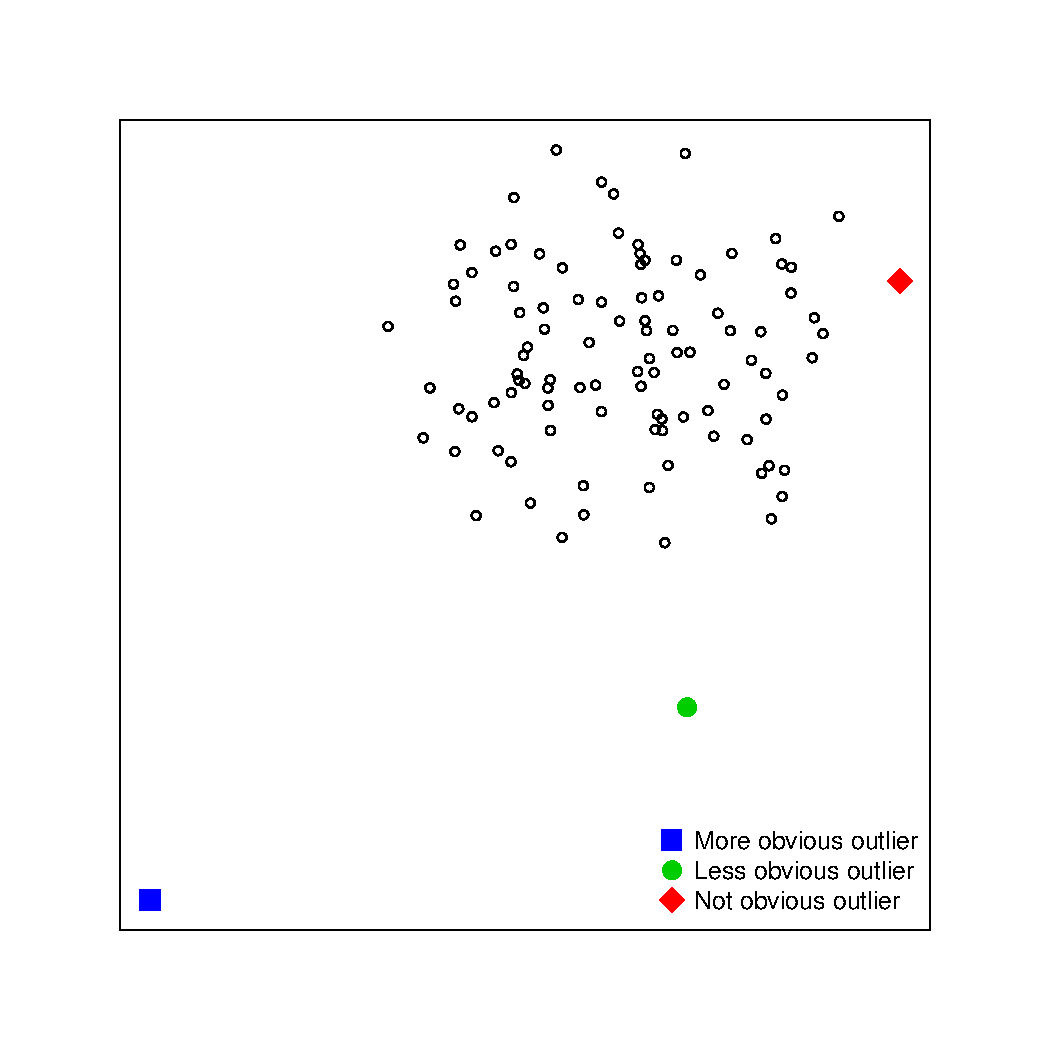
\includegraphics[width=4.7cm]{figs/data.pdf}}
\qquad
\subfloat[Individual separability curves]{\label{fig:ind_avg_curv} 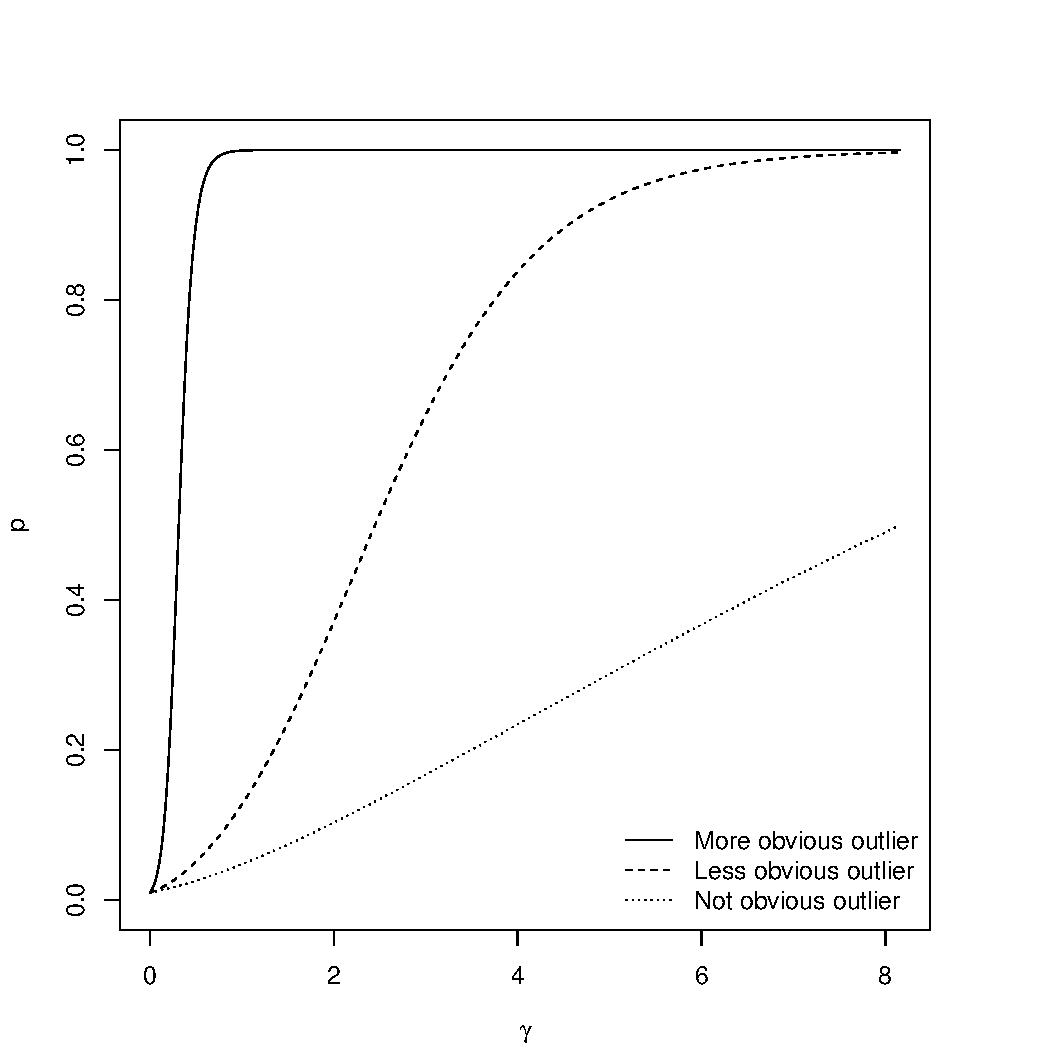
\includegraphics[width=4.7cm]{figs/sep_curves.pdf}}
\qquad
\subfloat[Weighted average curve of separability]{\label{fig:avg_sep_curv} 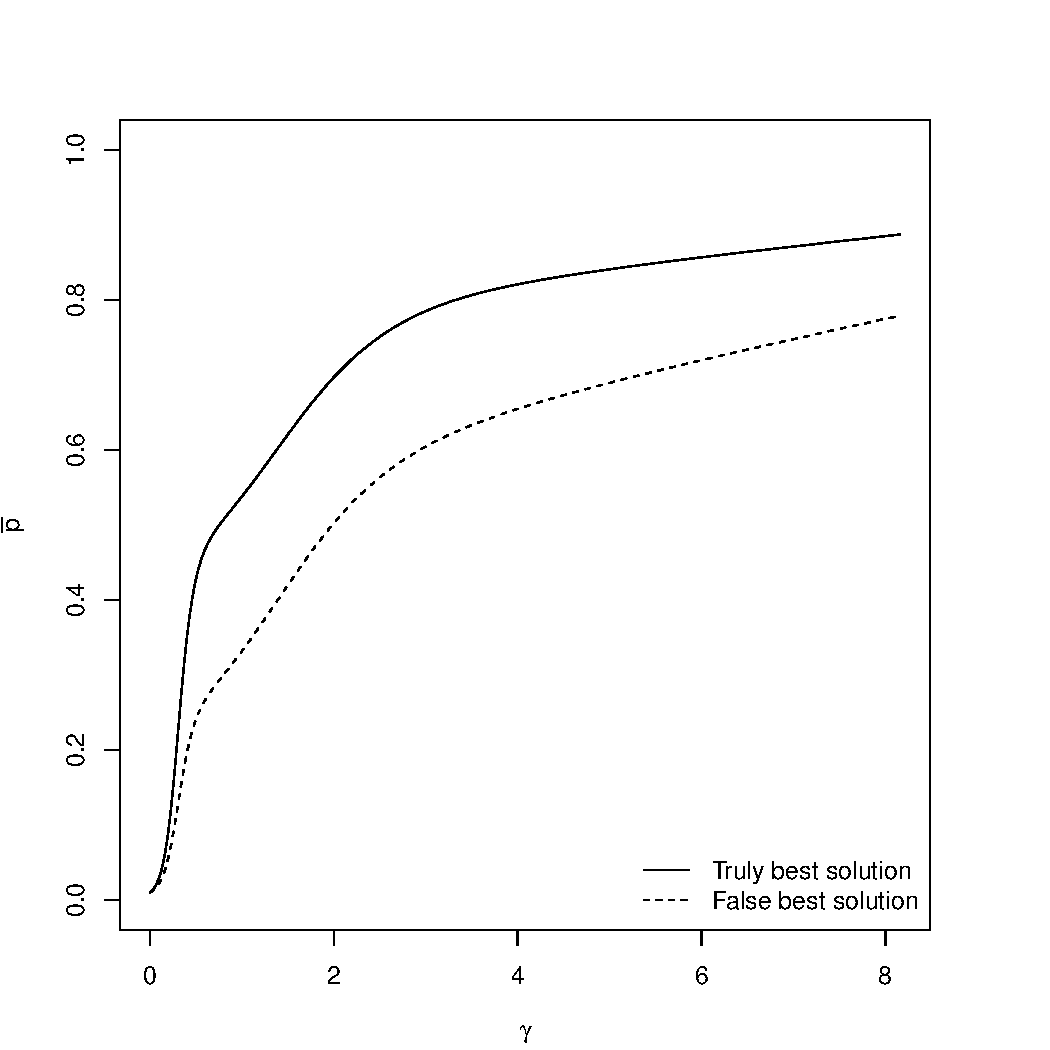
\includegraphics[width=4.7cm]{figs/avg_sep_curves.pdf}}
\caption{Illustrative example of a top-$n$ outlier solution: In \ref{fig:data} the top three observations are labeled as outliers; Their separabilities are individually assessed in \ref{fig:ind_avg_curv}; The outlier scorings of the two different top-$n$ solution are evaluated in \ref{fig:avg_sep_curv}, the outlier scores of the more obvious outlier, the less obvious outlier and not obvious outliers are respectively 1, 0.75, 0.51 for the truly best solution and 0.51, 0.75, 1 for the false best solution}
\label{fig:ilustration}
\end{figure}

The extension proposed here is computed similarly to the original index presented in the Equation \ref{eq:original_ireos}. However, instead of use the average curve of separability (Equation \ref{eq:ireos:avg_curve}) we use the weighted average curve of separability (Equation \ref{eq:w_avg_sep}):
\begin{equation}
I(\mathbf{S}) = \frac{1}{n_{\gamma}} \sum_{l = 1}^{n_{\gamma}} \left( \frac{1}{\sum_{\mathbf{x}_i \in \mathbf{S}} w_i} \sum_{\mathbf{x}_i \in \mathbf{S}} p(\mathbf{x}_i, \gamma_l) w_i \right)
\label{eq:ext_ireos}
\end{equation}

Note that giving the same scores for all observations labeled as outliers the index of the Equation \ref{eq:ext_ireos} will be reduced to the original index of the Equation \ref{eq:original_ireos}, where the followed assumption is that all the observations labeled are equally outliers.

\subsection{Internal Evaluation of Scoring Outlier Detection Results}
From the first extension is easy to note that such index could be trivially extended in order to evaluate the whole outlier scorings. As we intend to evaluate the solution without make the assumption that the number of outliers in the dataset is known, we take into account the whole dataset $\mathbf{X}$ in the evaluation, instead of the only top-$n$ outlier observations present in $\mathbf{S}$:
\begin{equation}
I(\mathbf{S}) = \frac{1}{n_{\gamma}} \sum_{l = 1}^{n_{\gamma}} \left( \frac{1}{\sum_{\mathbf{x}_i \in \mathbf{X}} w_i} \sum_{\mathbf{x}_i \in \mathbf{X}} p(\mathbf{x}_i, \gamma_l) w_i \right)
\end{equation}

Note that with the scoring normalization proposed by \cite{kriegel2011}, the outlier scores of the inliers is expected to be close to 0\footnote{with the proposed normalization by \cite{kriegel2011}, it will often be in fact 0}, therefore, they will affect very little in the quality of the solution.  Moreover, the exchange between observations with similar scores will be slightly penalized (\textit{e. g.} the exchange between clear outliers, or between clear inliers), while the exchange between observations with a great contrast in the outlier scorings will be highly penalized (\textit{e. g.} the exchange between a clear outlier and a clear inlier).

\subsubsection{Modeling clumps}
The possible presence of clumps in the data set induces IREOS to provide the users with an optional control mechanism to adjust their expectations about clump sizes. The maximum clump size ($m_{cl}$) is responsible for determine the fraction of the cost $C$ associated with soft margin classifier that the observations labeled as outliers will receive, this fraction of the penalty ($\beta$) determine how much these observations will individually affect the separabilities from each other. Originally, the observations labeled as inliers receive the full cost $C$ and the observations labeled as outliers a fraction $\beta$ of the this full cost. Being $\beta = \frac{1}{m_{cl}}$, so that, one needs $m_{cl}$ observations (a full clump) labeled as outliers to get the same impact as a single inlier. However, here it does not exist anymore the inliers and outliers labeling, instead, the degree of outlierness takes place. In order to extend IREOS to continue supporting the modeling clumps, the penalty cost associated with observations $\mathbf{x}_i$ ($C(\mathbf{x}_i)$) will be given according to their degree of outlierness:
%\begin{equation}
%C(\mathbf{x}_i) = C \times \left( \frac{1}{m_{cl}} \right)^{\left(1-\frac{rank(\mathbf{x}_i)}{N - 1}\right)}
%\end{equation}

\begin{equation}
C(\mathbf{x}_i) = C \cdot \beta^{w_i}
\end{equation}
where $\beta$ continue as $\beta = \frac{1}{m_{cl}}$ and ${w_i}$ is the normalized outlier score associated with the observation $\mathbf{x}_i$. Note that the modeling clumps is reduced to the one used before when all the inliers receive 0 as outlier scorings ($\beta^0 = 1$, full cost for inliers) and all the outliers receive 1 as the outlier scorings ($\beta^1 = \frac{1}{m_{cl}}$, $\frac{1}{m_{cl}}$ of the cost for outliers).

%Note that the index will be reduced again to the original index when all the inliers receive 0 as outlier scorings and all the outliers receive 1 as the outlier scorings.

%\subsubsection{Adjustment for Chance}
%\subsubsection{Complexity}
%\subsubsection{Approximate Computation}
%\subsubsection{Internal Evaluation of Ranking Outlier Detection Results}
%scorings não dizem muito, simples ranking tera peso linear qndo não é recomendado pq dos inliers q sao maioria
%gammaMax
\newpage